%% ALA @ AAMAS submission — AAMAS/ACM proceedings format.
%% Build on Overleaf (free): set main document to this file, compiler pdfLaTeX.
%% Double-blind: the `anonymous,review' options hide author identity for submission.
%% Remove `anonymous,review' for the camera-ready, and swap in the ALA copyright block.
\documentclass[sigconf,nonacm,anonymous,review]{acmart}

\usepackage{booktabs}
\usepackage{graphicx}
\usepackage{amsmath}

\settopmatter{printacmref=false}
\renewcommand\footnotetextcopyrightpermission[1]{}
\pagestyle{plain}

\begin{document}

\title{Selfishness as an Accident of Cooperation: How Reward Structure Shapes
Emergent Coordination in a Multi-Agent Survival Gridworld}

\author{Anonymous Author(s)}
\affiliation{%
  \institution{Submitted to ALA @ AAMAS}
  \country{}
}

\begin{abstract}
Does rewarding a team of reinforcement-learning agents for collective success make them
more cooperative? We study this in a controlled multi-agent survival gridworld in which the
reward structure is the \emph{only} independent variable: environment, architecture,
training algorithm, episode structure and random seeds are all held fixed. Four
decentralised agents with partial observability learn resource-gathering policies under
Proximal Policy Optimisation, over a one-parameter family of reward functions
$r_i = \alpha\, r_i^{\text{own}} + (1-\alpha)\,\bar r^{\text{team}}$ that interpolates from
purely selfish ($\alpha{=}1$) to purely cooperative team-average reward ($\alpha{=}0$).
Across five random seeds, an explicitly cooperative reward produces \emph{significantly
lower} efficiency, fairness and coordination than reward schemes that preserve individual
incentive ($p<0.001$, Cohen's $d = 4$--$6$ for selfish vs.\ cooperative). Sweeping $\alpha$
reveals why: performance is a saturating increasing function of individual-incentive weight,
rising steeply as soon as an agent's own contribution accounts for even a quarter of its
signal, then plateauing. The harm is therefore specific to \emph{pure} team-average reward,
which makes free-riding individually rational and maximises the credit-assignment problem;
a free-riding index computed independently of our performance metrics confirms this mechanism
directly. Finally, we show the effect is \emph{understated} by a common implementation choice:
replacing the shared policy with four independent learners leaves selfish agents unchanged
but causes the cooperative condition to collapse further still (efficiency $0.502\to0.169$),
because parameter sharing partially conceals the credit-assignment failure. Varying resource
density shows the effect is significant throughout but scales with competition: it is largest
under scarcity and nearly vanishes under abundance. Fair, efficient coordination emerges not
from a cooperative objective but as a side effect of individual self-interest.
\end{abstract}

\keywords{Multi-agent reinforcement learning, emergent cooperation, reward shaping,
social dilemmas, credit assignment, PPO}

\maketitle

\section{Introduction}
Intelligence rarely arises in isolation. Ant colonies, wolf packs and early human tribes all
exhibit sophisticated cooperative behaviour with no central controller. A long-standing
question in multi-agent artificial intelligence is how, and whether, such cooperation emerges
among self-interested learning agents~\cite{axelrod1984cooperation,leibo2017ssd}. An
intuitive hypothesis is that if we simply \emph{reward agents for collective success}, they
will learn to cooperate. This paper tests that hypothesis under controlled conditions and
finds it to be, at best, misleading.

We build a partially observable multi-agent survival gridworld and treat the reward function
as a controlled independent variable while holding everything else fixed. We compare a
\emph{selfish} reward (each agent is rewarded only for its own collection), a
\emph{cooperative} reward (all agents receive the team average), and a continuum of
\emph{mixed} rewards between them. Our central, counterintuitive finding is that the
explicitly cooperative reward yields the \emph{least} fair, least efficient and least
coordinated behaviour, and that this is not an artefact of a single run: it holds across
seeds with very large effect sizes, and a sweep of the mixing weight explains the mechanism.

\paragraph{Contributions.}
\begin{itemize}
  \item A controlled experimental design in which reward structure is isolated as the sole
  independent variable in a Dec-POMDP survival gridworld (Sec.~\ref{sec:env}--\ref{sec:method}).
  \item A statistically supported result (5 seeds, Welch $t$-tests, effect sizes): reward
  schemes that preserve individual incentive significantly outperform pure team-average
  reward on efficiency, fairness and coordination (Sec.~\ref{sec:results}).
  \item An $\alpha$-sweep that turns three discrete conditions into a dose--response curve and
  localises a ``knee'' near $\alpha\approx0.25$, showing the harm is specific to pure
  team-average reward and identifying the mechanism as credit assignment / free-riding,
  corroborated by a free-riding index that is independent of our performance metrics.
  \item An architecture ablation showing that \emph{parameter sharing masks the pathology}:
  with four independent learners the cooperative condition collapses far further
  (efficiency $0.502\to0.169$) while selfish is unaffected. MARL studies that share
  parameters may systematically understate the harm of purely cooperative reward.
  \item A resource-density sweep establishing a boundary condition: the effect holds at every
  density tested but scales with competition, being largest under scarcity and negligible
  under abundance.
\end{itemize}

\section{Related Work}
\paragraph{Sequential social dilemmas.} Our setting is a sequential social
dilemma~\cite{leibo2017ssd}, where individually rational behaviour can undermine collective
outcomes, extending matrix-game dilemmas to temporally and spatially extended
environments. P{\'e}rolat et al.~\cite{perolat2017commons} study common-pool resource
appropriation and the tragedy of the commons~\cite{hardin1968tragedy} in a MARL setting;
Hughes et al.~\cite{hughes2018inequity} show inequity aversion can improve cooperation. Unlike
these works, which fix a reward regime and study behaviour, we treat the reward regime itself
as the manipulated variable and measure its causal effect.

\paragraph{Cooperative MARL and credit assignment.} Centralised-training / decentralised-
execution methods such as MADDPG~\cite{lowe2017maddpg}, COMA~\cite{foerster2018coma} and
MAPPO~\cite{yu2022mappo} target the credit-assignment problem directly. Our team-average
condition instead exposes credit assignment in its rawest form: with a shared reward and no
counterfactual baseline, an agent cannot tell whether its own actions produced reward. We use
PPO~\cite{schulman2017ppo} with generalised advantage estimation~\cite{schulman2016gae} as a
deliberately simple, interpretable learner rather than a state-of-the-art cooperative method.

\paragraph{Environments.} Standard MARL benchmarks are not designed to vary the reward regime
as a control: SMAC~\cite{samvelyan2019smac} is purely cooperative, and the multi-agent
particle environments accessed via PettingZoo~\cite{terry2021pettingzoo} do not expose a
configurable selfish/cooperative axis. Our environment is built specifically so that only the
reward transformation differs across conditions.

\section{Environment}
\label{sec:env}
The environment is a $25\times25$ discrete grid masked to an octagonal arena (to avoid corner
bias). It hosts $N=4$ agents, $25$ resource nodes, and $45$ static obstacles. Resources
regenerate slowly: at each step, with probability $0.02$, one resource respawns at a random
free cell, subject to a cap at the initial resource count. Over a $250$-step episode this adds
roughly five resources, so the environment never becomes static but scarcity is preserved. Each agent observes only a $5\times5$
local window centred on itself, flattened to a $25$-dimensional integer vector; it never
observes the global state. Actions are the five moves \{stay, up, down, left, right\};
collisions with walls, obstacles and other agents leave the agent in place. Episodes run for
$250$ steps (truncation) or until all resources are depleted (termination).

Formally the system is a decentralised partially observable Markov decision process
$\langle N, S, \{A_i\}, T, \{R_i\}, \{\Omega_i\}, \{O_i\}, \gamma\rangle$ with $N=4$,
$\gamma=0.99$, stochastic transitions $T$ (resource respawn), and observation function $O_i$
mapping the global state to agent $i$'s local window. Crucially, the components differ across
our experimental conditions \emph{only} in the reward functions $\{R_i\}$.

\section{Method}
\label{sec:method}
\paragraph{Learner.} All agents share a single PPO policy (parameter sharing): a two-layer MLP
with $64$ hidden units per layer and ReLU activations, and separate policy and value heads.
We use GAE ($\lambda=0.95$), a clipped objective ($\epsilon=0.2$), entropy regularisation
($0.01$), value loss coefficient $0.5$, gradient-norm clipping ($0.5$), and Adam
($3\times10^{-4}$). The four agents contribute to a single shared PPO buffer, updated at the
end of each episode. The small network is a deliberate choice: the research question concerns
how reward structure shapes behaviour, not maximal performance, and a simple learner yields
more interpretable behaviour.

\paragraph{The reward family.} The environment emits a raw individual signal
$r_i^{\text{own}}\in\{0,1\}$ (1 when agent $i$ collects a resource). A reward manager
transforms this into the delivered reward without altering the environment:
\begin{equation}
  r_i \;=\; \alpha\, r_i^{\text{own}} \;+\; (1-\alpha)\,\bar r^{\text{team}},
  \qquad \bar r^{\text{team}} = \tfrac{1}{N}\textstyle\sum_j r_j^{\text{own}}.
  \label{eq:reward}
\end{equation}
This single parameter spans our conditions: $\alpha{=}1$ is \emph{selfish} (own reward only),
$\alpha{=}0$ is \emph{cooperative} (pure team average, Eq.~\eqref{eq:reward} with no individual
term), and $\alpha{=}0.5$ is the \emph{mixed} midpoint. No cooperative behaviour is ever
programmed; any coordination must emerge from learning.

\paragraph{Methodological fixes.} To make the study reproducible and the comparison valid, we
(i) seed Python, NumPy \emph{and} PyTorch weight initialisation from a single master seed, so
conditions differ only in reward; (ii) bootstrap the value target from $V(s_T)$ on the
$250$-step truncation rather than treating it as a terminal state; and (iii) use the pure
team-average form for the cooperative condition, matching Eq.~\eqref{eq:reward} at $\alpha{=}0$.

\section{Experimental Setup}
\label{sec:setup}
We train each condition for $30{,}000$ episodes on CPU, repeated over $5$ random seeds
(the $\alpha$-sweep and the architecture ablation use $3$ seeds). A single master seed
controls Python, NumPy and PyTorch weight initialisation, so conditions differ only in reward. We report four metrics over the final $100$ episodes:
mean total reward; \emph{efficiency} (resources collected $/$ resources spawned);
\emph{Jain fairness}~\cite{jain1984fairness} over per-agent collection counts; and a
\emph{cooperation score} defined as efficiency $\times$ fairness. Because that score is by
construction not independent of the other two, we additionally report two direct measures of
free-riding: the \emph{free-rider fraction} (mean fraction of agents collecting less than half
the per-episode per-agent mean) and the \emph{contribution Gini} over per-agent collection
counts. We report mean $\pm$ standard deviation across seeds and assess pairwise differences
with two-sided Welch $t$-tests and Cohen's $d$.

\section{Results}
\label{sec:results}

\begin{table}[t]
\caption{Final-100-episode metrics, mean $\pm$ s.d.\ over 5 seeds. Best per row in bold.}
\label{tab:main}
\begin{tabular}{lccc}
\toprule
Metric & Selfish & Cooperative & Mixed \\
\midrule
Efficiency    & \textbf{0.627 $\pm$ 0.032} & 0.502 $\pm$ 0.027 & 0.584 $\pm$ 0.045 \\
Jain fairness & \textbf{0.716 $\pm$ 0.013} & 0.656 $\pm$ 0.005 & 0.692 $\pm$ 0.016 \\
Cooperation   & \textbf{0.455 $\pm$ 0.028} & 0.338 $\pm$ 0.015 & 0.410 $\pm$ 0.035 \\
Reward        & \textbf{15.67 $\pm$ 0.81}  & 12.56 $\pm$ 0.67  & 14.60 $\pm$ 1.12  \\
\bottomrule
\end{tabular}
\end{table}

\paragraph{Cooperative reward is significantly worse.}
Table~\ref{tab:main} shows the headline result. Selfish reward beats cooperative reward on
every metric, with very large effect sizes: efficiency ($p=0.0002$, $d=4.2$), fairness
($p=0.0001$, $d=6.2$) and cooperation ($p=0.0002$, $d=5.1$). The cooperative condition is also
significantly worse than mixed ($p<0.05$ on all three metrics). By contrast, selfish and mixed
are statistically close (efficiency $p=0.12$, cooperation $p=0.06$; both n.s., and fairness
also non-significant once corrected for multiple comparisons). The defensible claim is
therefore $\{\text{selfish},\text{mixed}\} \gg \text{cooperative}$, rather than a strict
three-way ordering. All conclusions in this paragraph survive Holm--Bonferroni correction
across the nine-test family (Appendix~\ref{app:repro}).

\paragraph{Learning dynamics.}
Figure~\ref{fig:curves} shows why the averages differ. Selfish and mixed recover quickly to a
stable plateau; the cooperative condition collapses early --- when all agents are near-random,
the shared reward is extremely noisy and an agent is rewarded for teammates' collections it
did not cause --- and recovers only slowly. This is the credit-assignment problem manifesting
as an extended period of near-random exploration. The across-seed bands for cooperative remain
separated from the other two throughout, visually confirming the significance tests.

\begin{figure}[t]
\centering
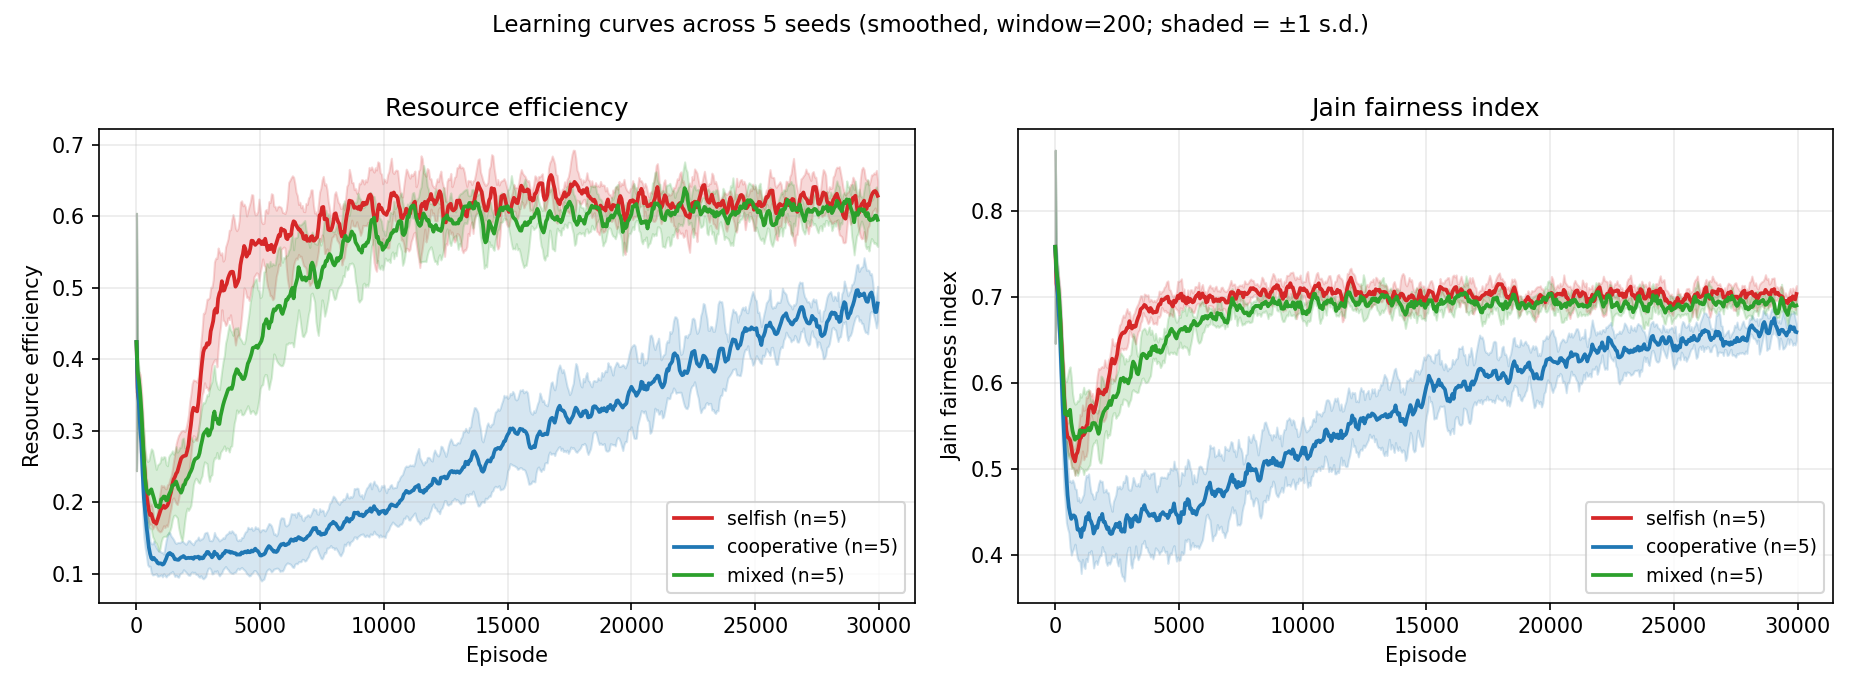
\includegraphics[width=\linewidth]{figures/learning_curves.png}
\caption{Learning curves across 5 seeds (smoothed; shaded $=\pm1$ s.d.). Cooperative (blue)
collapses and recovers slowly; selfish (red) and mixed (green) overlap but dominate throughout.}
\label{fig:curves}
\end{figure}

\paragraph{The mechanism: an $\alpha$-sweep.}
Figure~\ref{fig:alpha} sweeps the mixing weight of Eq.~\eqref{eq:reward}. All three metrics rise
steeply as $\alpha$ increases from $0$ (cooperative) to $0.25$, then plateau: on efficiency,
$+0.090$ from $\alpha{=}0$ to $0.25$ but only $+0.038$ more across $0.25$ to $1$. The harm is
thus specific to \emph{pure} team-average reward; as soon as an agent's own contribution is
even a quarter of its signal, free-riding ceases to be individually rational and performance
jumps. As a consistency check, the standalone selfish and cooperative runs (hollow squares)
coincide exactly with the $\alpha{=}1$ and $\alpha{=}0$ endpoints of the swept curve --- indeed
they are byte-identical per seed, since Eq.~\eqref{eq:reward} reduces to those conditions.

\begin{figure}[t]
\centering
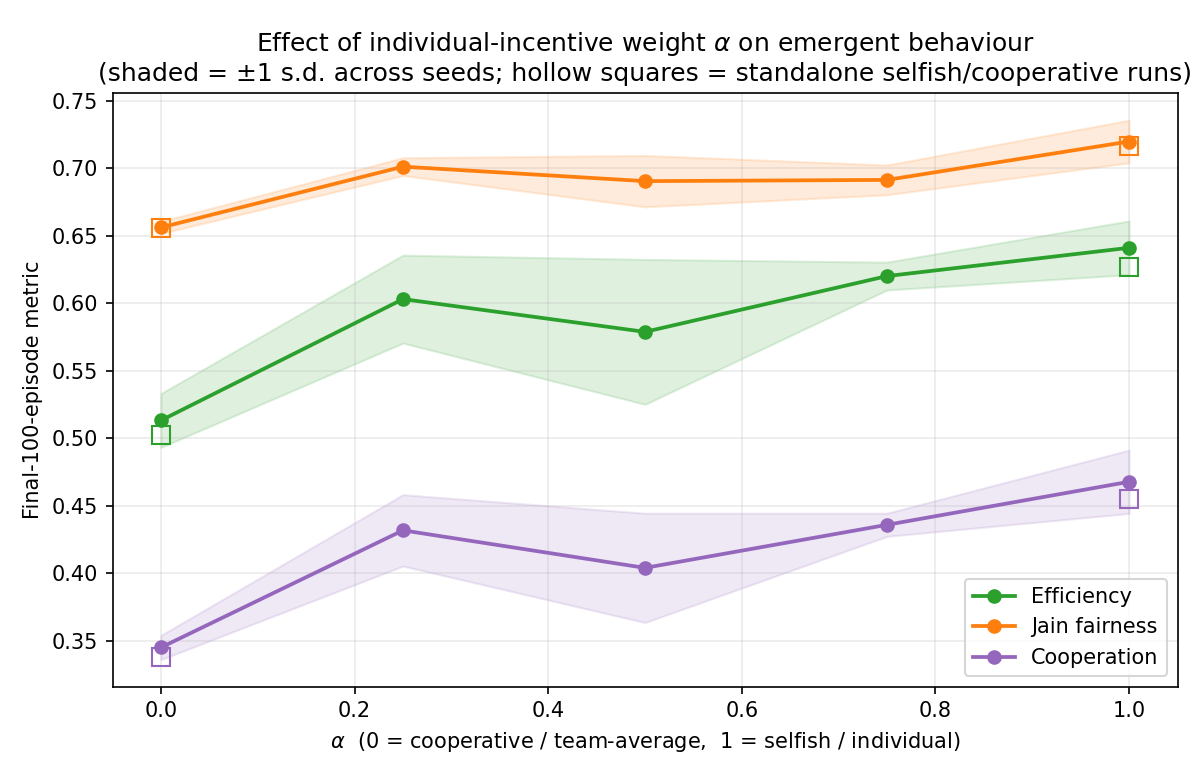
\includegraphics[width=\linewidth]{figures/alpha_sweep.png}
\caption{Effect of individual-incentive weight $\alpha$ (0 = cooperative, 1 = selfish).
Metrics saturate: the knee is near $\alpha\approx0.25$. Hollow squares are the standalone
selfish/cooperative runs, landing on the curve endpoints.}
\label{fig:alpha}
\end{figure}

\paragraph{Direct evidence of free-riding.}
The mechanism we posit --- that team-average reward makes contributing optional --- predicts
measurably more free-riding under the cooperative condition. Table~\ref{tab:freerider} confirms
this with measures that do not depend on our efficiency/fairness product. Under cooperative
reward, $30.7\%$ of agents collect less than half the per-agent mean, against $25.1\%$ under
selfish ($p=0.002$, $d=3.0$), and contribution inequality is significantly higher
($p=0.0002$, $d=6.0$). Cooperative reward also free-rides significantly more than mixed on both
measures. This is direct behavioural evidence for the credit-assignment account, rather than a
restatement of the headline metrics.

\begin{table}[t]
\caption{Free-riding measures (final 100 episodes, mean $\pm$ s.d.\ over 5 seeds).
Higher = more free-riding. Cooperative is worst on both.}
\label{tab:freerider}
\begin{tabular}{lccc}
\toprule
Measure & Selfish & Cooperative & Mixed \\
\midrule
Free-rider fraction & \textbf{0.251 $\pm$ 0.015} & 0.307 $\pm$ 0.022 & 0.275 $\pm$ 0.014 \\
Contribution Gini   & \textbf{0.331 $\pm$ 0.012} & 0.384 $\pm$ 0.005 & 0.351 $\pm$ 0.014 \\
\bottomrule
\end{tabular}
\end{table}

\paragraph{Parameter sharing masks the pathology.}
Our main experiments share one policy across the four agents, a near-ubiquitous convenience in
MARL. To test whether this drives the result, we repeat the selfish and cooperative conditions
with \emph{four fully independent learners} (a separate network and optimiser per agent),
changing nothing else. The outcome, in Fig.~\ref{fig:ablation} and Table~\ref{tab:ablation},
is asymmetric and striking. Selfish agents are \emph{unaffected}: efficiency
$0.627\to0.638$ ($p=0.70$, n.s.). The cooperative condition collapses: efficiency
$0.502\to0.169$, reward $12.56\to4.23$. The selfish--cooperative efficiency gap widens from
$0.125$ to $0.469$ ($p=0.0004$, $d=14.5$), and the free-rider fraction rises from $0.307$ to
$0.418$ ($p<0.05$, $d=3.4$).

The explanation follows from the credit-assignment account. With a shared policy, all four
agents' transitions update one network, so even under team-average reward that network still
observes that collecting produces reward --- a single policy cannot free-ride on itself.
Give each agent its own parameters and the team-average signal becomes nearly uncorrelated
with that agent's own actions; free-riding becomes individually learnable, and the system
degrades toward passivity. Indeed the independent cooperative agents finish \emph{below} the
near-random return of early training, i.e.\ they have learned to do less than a random policy.
The practical implication is that parameter sharing partially conceals this failure mode:
studies that share parameters may systematically \emph{understate} how harmful a purely
cooperative reward is.

\begin{figure}[t]
\centering
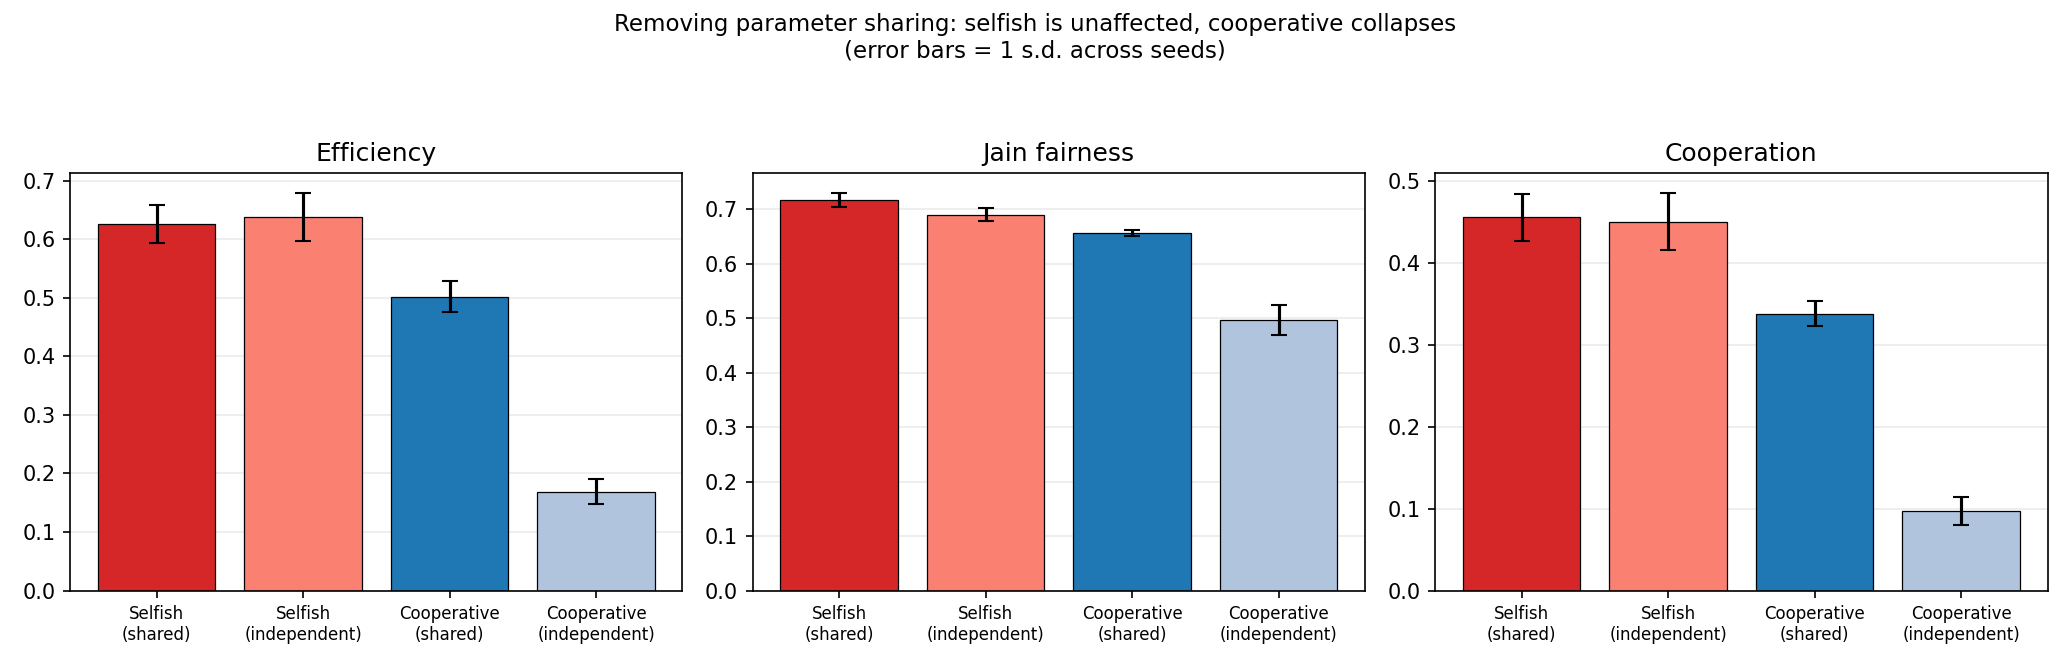
\includegraphics[width=\linewidth]{figures/ablation.png}
\caption{Removing parameter sharing. Selfish (red) is unchanged; cooperative (blue) collapses.
Error bars are 1 s.d.\ across seeds.}
\label{fig:ablation}
\end{figure}

\begin{table}[t]
\caption{Shared-weight vs.\ independent learners (mean $\pm$ s.d.). Selfish is unaffected;
cooperative collapses.}
\label{tab:ablation}
\begin{tabular}{lcccc}
\toprule
& \multicolumn{2}{c}{Selfish} & \multicolumn{2}{c}{Cooperative} \\
\cmidrule(lr){2-3}\cmidrule(lr){4-5}
Metric & shared & indep. & shared & indep. \\
\midrule
Efficiency    & 0.627 & 0.638 & 0.502 & \textbf{0.169} \\
Jain fairness & 0.716 & 0.690 & 0.656 & \textbf{0.496} \\
Cooperation   & 0.455 & 0.450 & 0.338 & \textbf{0.097} \\
Free-rider frac. & 0.251 & 0.278 & 0.307 & \textbf{0.418} \\
\bottomrule
\end{tabular}
\end{table}

\paragraph{The effect is modulated by scarcity.}
To test whether our finding is specific to one level of competition, we repeat the selfish and
cooperative conditions at $15$ and $40$ resources (vs.\ the default $25$), normalising
efficiency by each run's own resource count. Figure~\ref{fig:density} shows the outcome.
Selfish agents are remarkably insensitive to scarcity, collecting a near-constant proportion
of the initial resource pool ($0.619 \to 0.648$ efficiency across a $2.7\times$ change in
resources).\footnote{Because respawn contributes a roughly fixed number of additional
resources per episode regardless of density, absolute efficiency values are not perfectly
comparable across densities. The selfish--cooperative \emph{gap} at a given density is
unaffected, since both conditions share the same denominator; our claims concern those gaps.}
Cooperative agents are fragile: efficiency nearly doubles from scarce to abundant
($0.297 \to 0.570$). Consequently the selfish--cooperative gap falls monotonically as
resources become plentiful --- efficiency $+0.322 \to +0.125 \to +0.078$, and the fairness gap
all but disappears under abundance ($+0.127 \to +0.060 \to +0.009$). The difference remains
statistically significant at every density tested ($p=0.0012$, $0.0002$, $0.0187$
respectively), so the result generalises; what changes is its magnitude.

This is precisely what a social-dilemma account predicts. Scarcity is what gives free-riding
its cost: when resources are abundant there is enough for everyone regardless of how work is
distributed, so a passive agent barely harms the group. As resources contract, the same
free-riding becomes ruinous. Our finding is therefore not a universal claim but one with a
stated boundary condition: \emph{team-average reward is largely benign under abundance and
increasingly harmful under competition}.

\begin{figure}[t]
\centering
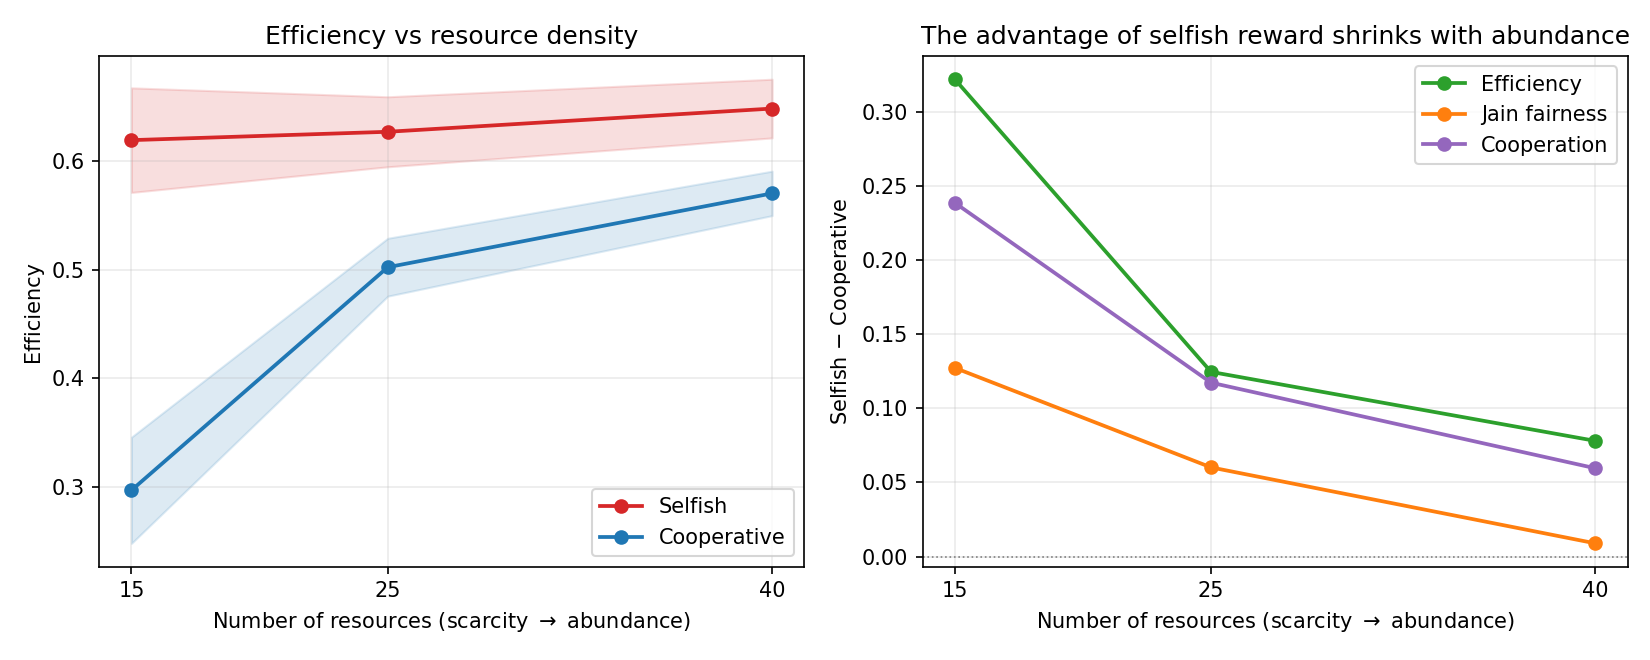
\includegraphics[width=\linewidth]{figures/density.png}
\caption{Resource-density sweep. Left: selfish efficiency (red) is near-constant while
cooperative (blue) degrades sharply under scarcity; shaded $=\pm1$ s.d. Right: the
selfish-minus-cooperative gap shrinks monotonically as resources become abundant.}
\label{fig:density}
\end{figure}

\paragraph{Qualitative behaviour.}
Under selfish reward, agents develop distinct spatial territories (Fig.~\ref{fig:qual}); this
is not motivated by fairness but is the individually rational response to competition, and it
produces fair collection counts as a side effect --- a correlated equilibrium reached without
communication or shared objective.

\begin{figure}[t]
\centering
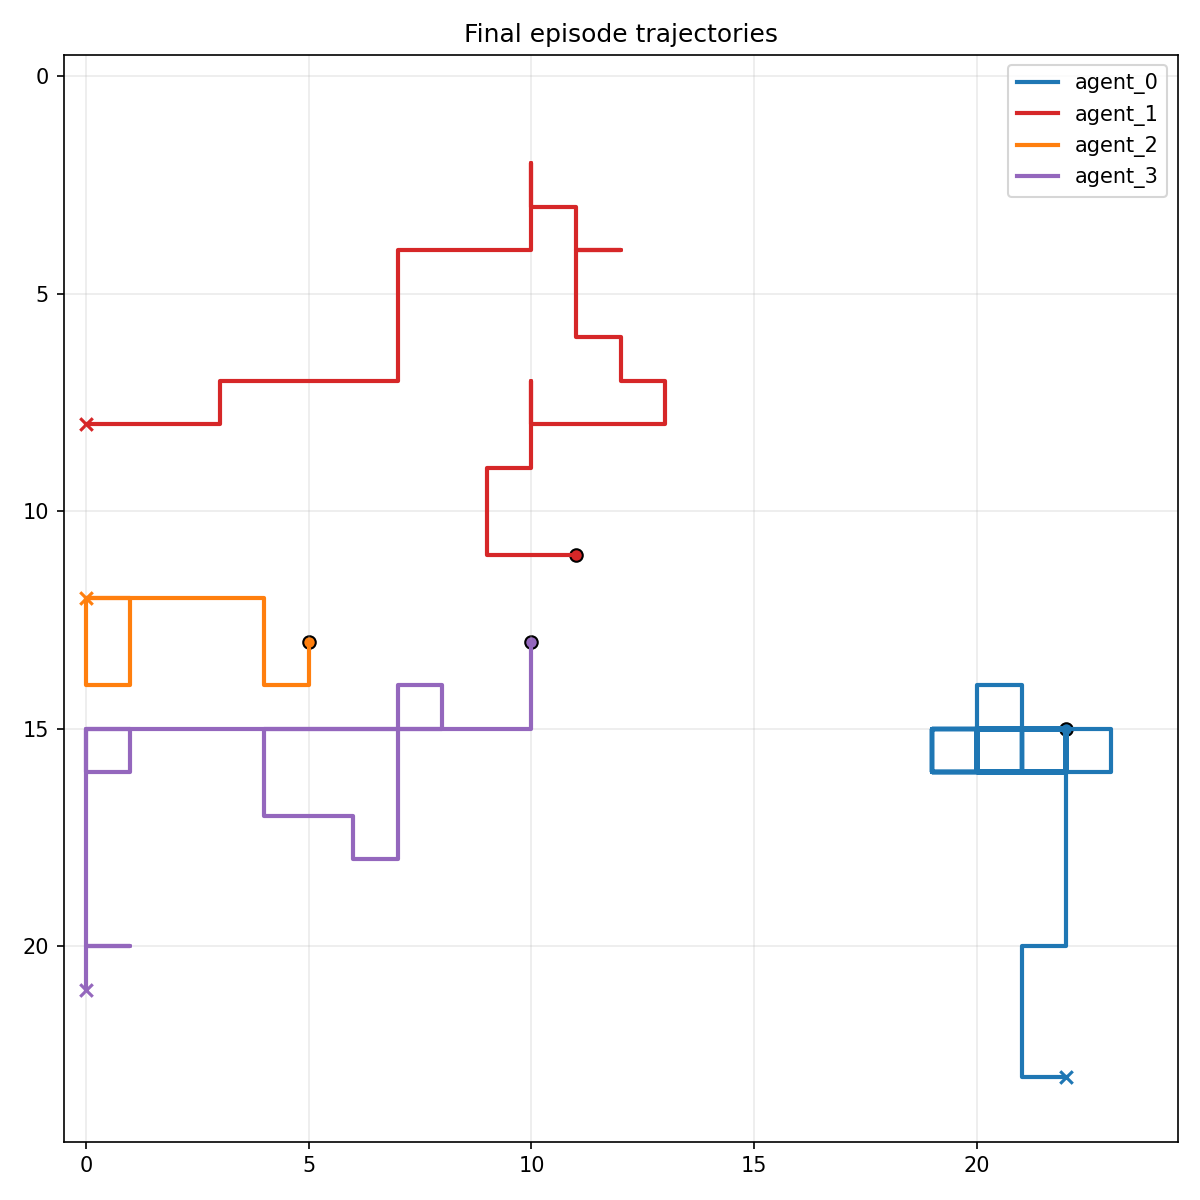
\includegraphics[width=0.48\linewidth]{figures/trajectory_selfish.png}
\hfill
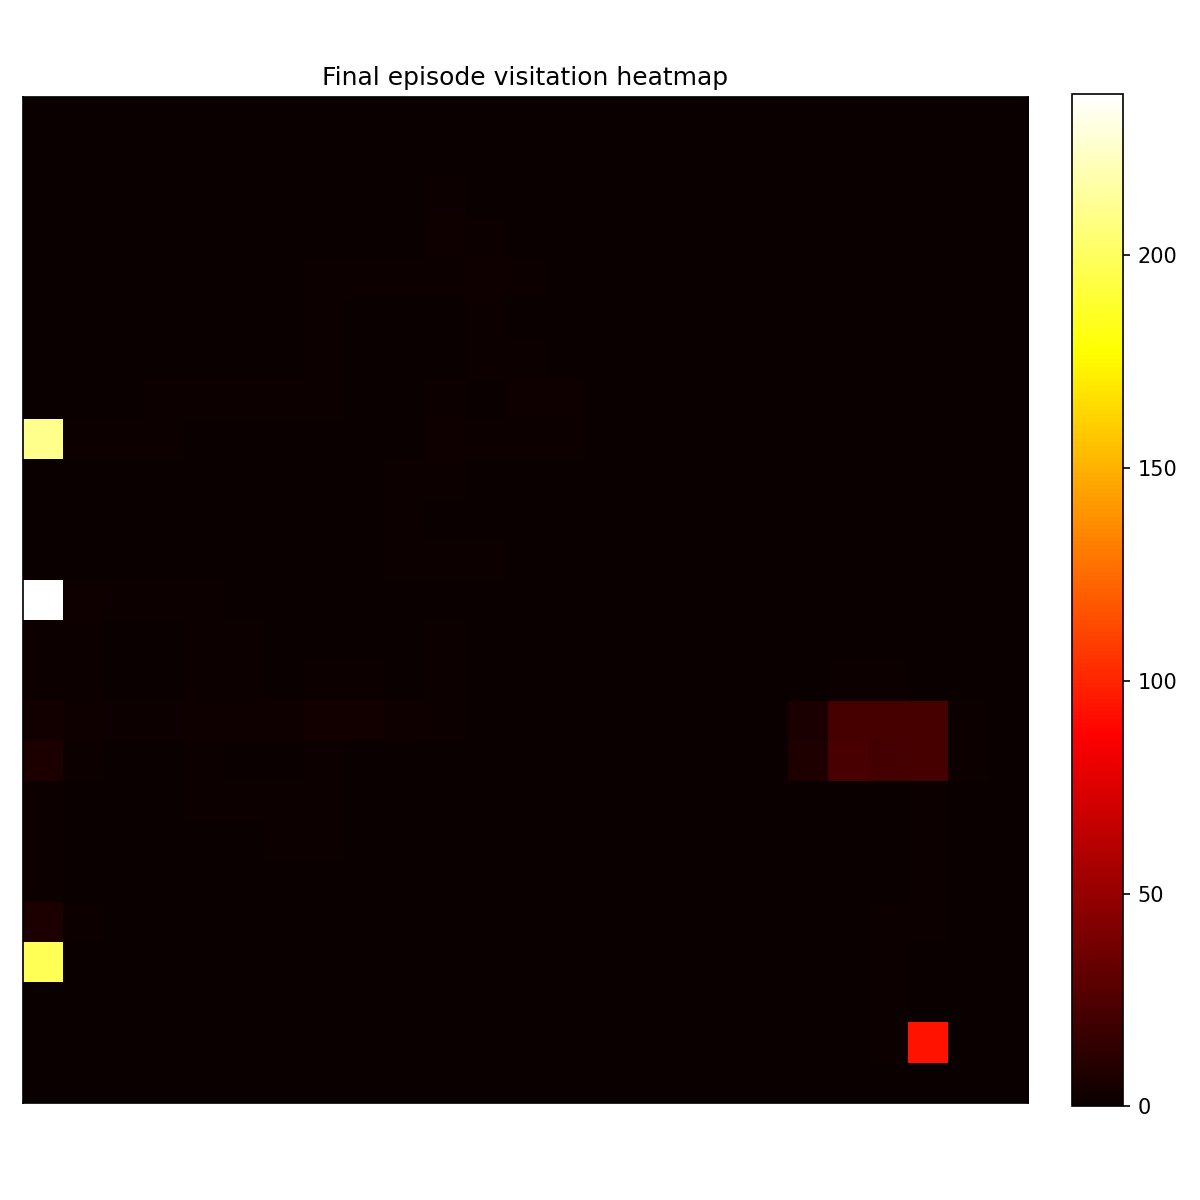
\includegraphics[width=0.48\linewidth]{figures/heatmap_selfish.png}
\caption{Emergent territorial separation under selfish reward: agent trajectories (left) and
average visitation heatmap (right).}
\label{fig:qual}
\end{figure}

\section{Discussion}
Our results connect directly to the tragedy of the commons and the Prisoner's
Dilemma~\cite{hardin1968tragedy,axelrod1984cooperation}. Pure team-average reward removes the
punishment for defection: an agent that contributes nothing still receives the team average,
so free-riding is rational and the cooperative equilibrium is unstable. Selfish reward, by
contrast, makes inaction immediately costly, and the individually rational strategy
(spreading out to avoid competition) happens to be collectively beneficial. Cooperation, in
this environment, is best understood as an accidental by-product of self-interest rather than
a behaviour that a cooperative objective reliably induces.

\paragraph{Threats to validity.} The shared-weight concern is addressed directly by our
ablation, which shows the effect strengthens rather than disappears without parameter
sharing, and the single-configuration concern by the density sweep, which finds the effect at
every density tested. Generalisation across agent counts remains open: whether the effect grows
with team size --- as the credit-assignment account predicts, since each agent's share of the
team average shrinks as $1/N$ --- is untested here and is the most direct next experiment. The cooperation score is not independent of
efficiency and fairness, which is why we also report the free-rider fraction and contribution
Gini. We use $5$ seeds ($3$ for the $\alpha$-sweep, ablation and density runs); the ablation's effect sizes
($d>9$ on every metric) are large enough that this is not a practical concern. The most
important open question is whether a centralised critic~\cite{yu2022mappo,foerster2018coma},
designed precisely to solve credit assignment, repairs the cooperative condition. Our account
predicts it should substantially help, which would make the failure mode a property of naive
independent learners rather than of cooperative reward as such.

\section{Conclusion}
Rewarding agents for collective success does not reliably produce cooperation; in our
controlled study it does the opposite, significantly harming fairness, efficiency and
coordination relative to reward schemes that preserve individual incentive, and it does so
more severely once the convenience of parameter sharing is removed. An $\alpha$-sweep
localises the harm to pure team-average reward and identifies credit assignment as the cause.
The most promising next steps are a centralised-critic baseline and generalisation across agent
counts and resource densities.

\bibliographystyle{ACM-Reference-Format}
\bibliography{references}

\appendix

\section{Reproducibility}
\label{app:repro}

\paragraph{Code and data.} All code, run configurations and analysis scripts are released with
the paper. Every number reported traces to a logged run: each run writes a per-episode CSV, a
per-episode JSON metric log, and a \texttt{summary.json} of the final-100-episode statistics.
The aggregation, significance testing and every figure are regenerated from those files by the
released scripts, with no manual transcription.

\paragraph{Environment configuration.} $25\times25$ grid with an octagonal playable mask;
$N=4$ agents; $25$ resource nodes; $45$ static obstacles; resource respawn probability
$0.02$ per step (a single respawn attempt per step, capped at the initial resource count);
$5\times5$ egocentric observation window (flattened to
$25$ integers); $5$ discrete actions (stay, up, down, left, right); episode limit $250$ steps
(truncation) or resource exhaustion (termination). Obstacle, resource and agent placements are
randomised per episode from the episode seed.

\paragraph{PPO hyperparameters.} $\gamma=0.99$; GAE $\lambda=0.95$; clip ratio $0.2$;
Adam learning rate $3\times10^{-4}$; $4$ epochs per update; minibatch size $64$; value loss
coefficient $0.5$; entropy coefficient $0.01$; gradient-norm clip $0.5$. Policy/value network:
shared two-layer MLP ($64$ units, ReLU) with separate linear policy ($\rightarrow 5$) and value
($\rightarrow 1$) heads. Updates occur at the end of each episode from a buffer holding all
four agents' transitions, with advantages computed per agent trajectory. On truncation the
value target bootstraps from $V(s_T)$; only genuine termination is treated as terminal.

\paragraph{Seeding.} A single master seed sets Python's \texttt{random}, NumPy and PyTorch
weight initialisation. Episode seeds are drawn from a disjoint per-seed stream
($\text{seed}\times N_{\text{episodes}} + \text{episode}$) so that no two runs share an episode
sequence. Main conditions use seeds $0$--$4$; the $\alpha$-sweep and the architecture ablation
use seeds $0$--$2$.

\paragraph{Compute.} All experiments run on CPU on a single Apple M1 laptop (4 performance
cores), with no GPU. Runs are executed single-threaded, four concurrently. A $30{,}000$-episode
shared-weight run takes roughly $2.5$ hours; independent-learner runs are slower (four networks
per update). The full set reported here --- $15$ main runs, $15$ $\alpha$-sweep runs and $6$
ablation runs --- totals under $30$ hours of wall-clock time. No paid or cloud compute was used.

\paragraph{Software.} Python 3.14, PyTorch 2.11, NumPy 2.4, PettingZoo 1.24 (the environment
implements the \texttt{ParallelEnv} API). PPO is implemented from scratch rather than taken
from an RL library, so that trajectory buffering and per-agent advantage computation are fully
specified by the released code.

\paragraph{Metric definitions.} Efficiency is total resources collected divided by resources
spawned ($25$). Jain fairness~\cite{jain1984fairness} is computed over the four per-agent
collection counts of an episode. The cooperation score is their product. The free-rider
fraction is the mean fraction of agents whose collection falls below half the per-episode
per-agent mean; the contribution Gini is the Gini coefficient of the per-agent counts. All
are averaged over the final $100$ episodes of a run, then aggregated across seeds.

\paragraph{Statistics.} Group comparisons use two-sided Welch $t$-tests on per-seed
final-100-episode means (i.e.\ $n$ equals the number of seeds, not episodes), with Cohen's $d$
computed from the pooled standard deviation. We report exact $p$-values and effect sizes rather
than significance thresholds alone. Because the main comparison involves nine tests (three
metrics $\times$ three condition pairs), we additionally apply a Holm--Bonferroni correction to
that family. All selfish-vs-cooperative comparisons remain significant
($p_{\text{adj}}\le0.0016$), as do all cooperative-vs-mixed comparisons
($p_{\text{adj}}\le0.0444$); every selfish-vs-mixed comparison is non-significant after
correction. The correction therefore supports exactly the claim we make in
Sec.~\ref{sec:results}, and we report uncorrected values in the main text for transparency.

\end{document}
